\documentclass[10pt]{article}\usepackage[margin=18mm]{geometry}\usepackage{graphicx}\usepackage{hyperref}\usepackage{float}\setlength{\parskip}{5pt}\setlength{\parindent}{0pt}\title{Frozen V3/V4 Descriptor and Probabilistic World-Model Validation}\author{Strictly offline local audit}\date{2026-07-12}\begin{document}\maketitle\section{Decision}Decision C - descriptor semantics incomplete or inconsistent is the single main decision. Strict spatial extrapolation and topology-mask support are inadequate for an EIG pilot.\section{Scope}No exact solver, Delta-q search, active-learning loop, HPC job, or frozen-data edit was performed. Historical learned state is non-transferable.\section{Method}Inputs are $(k_BT/t,J_A/t,\mu/t)$. Outputs use fixed physical transforms and field-specific applicability/reliability masks. Normal-state $q$ is not applicable, never a valid zero. Spatial, slice, corner, future, cross-run, probe-cloud, sequential replay, and retrospective tests were run.\section{Results}See the machine-readable CSV companions for per-field MAE, RMSE, $R^2$, NLL, interval coverage, uncertainty-error correlation, and replay/control values.\clearpage\begin{figure}[p]\centering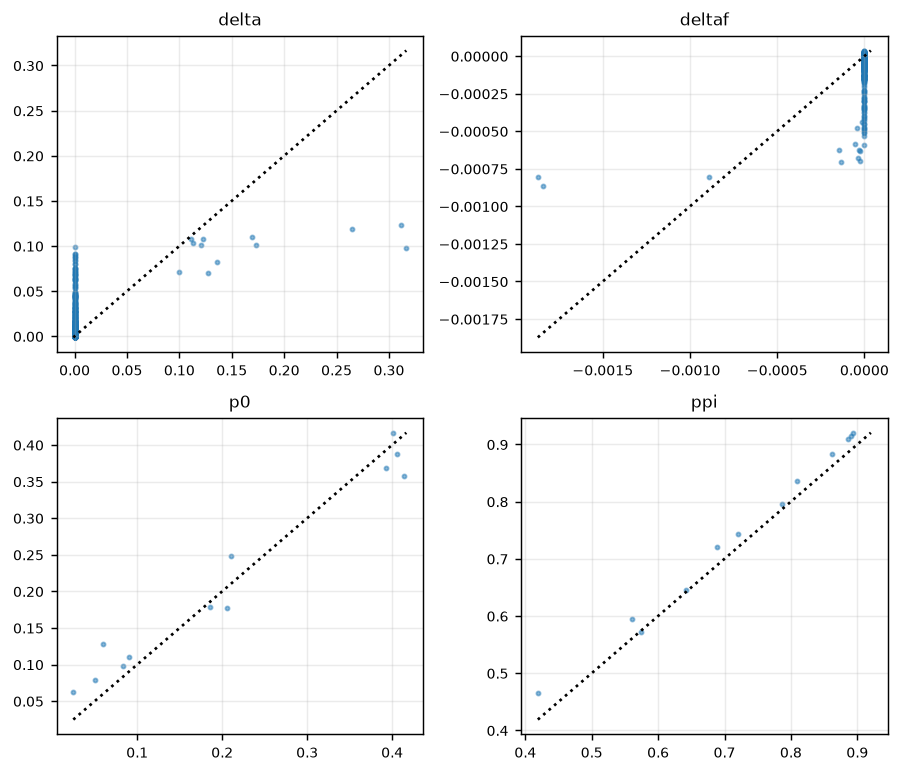
\includegraphics[width=.92\textwidth]{../figures/figure_01_predicted_exact.png}\caption{figure 01 predicted exact}\end{figure}
\begin{figure}[p]\centering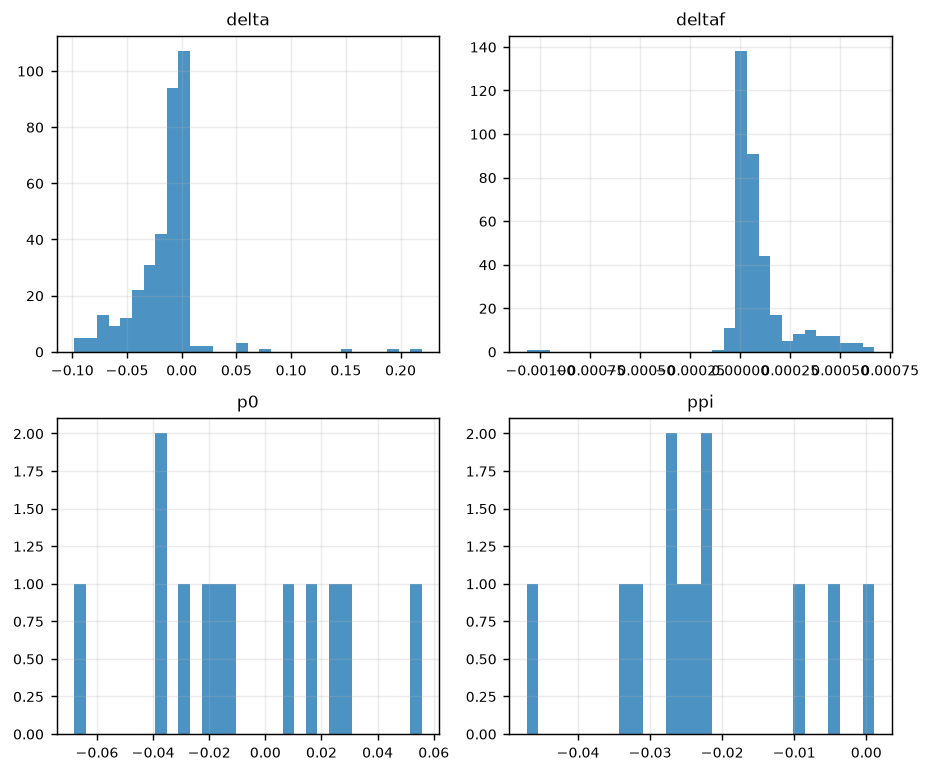
\includegraphics[width=.92\textwidth]{../figures/figure_02_residuals.png}\caption{figure 02 residuals}\end{figure}
\begin{figure}[p]\centering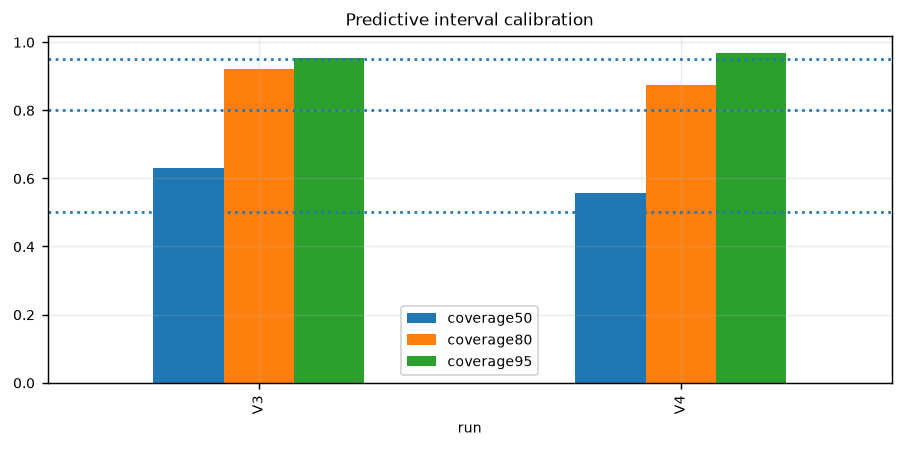
\includegraphics[width=.92\textwidth]{../figures/figure_03_calibration.png}\caption{figure 03 calibration}\end{figure}
\begin{figure}[p]\centering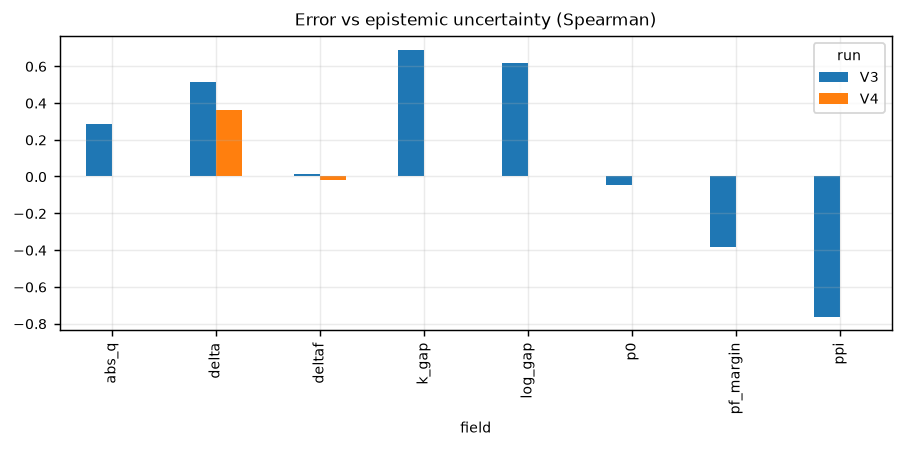
\includegraphics[width=.92\textwidth]{../figures/figure_04_error_epistemic.png}\caption{figure 04 error epistemic}\end{figure}
\begin{figure}[p]\centering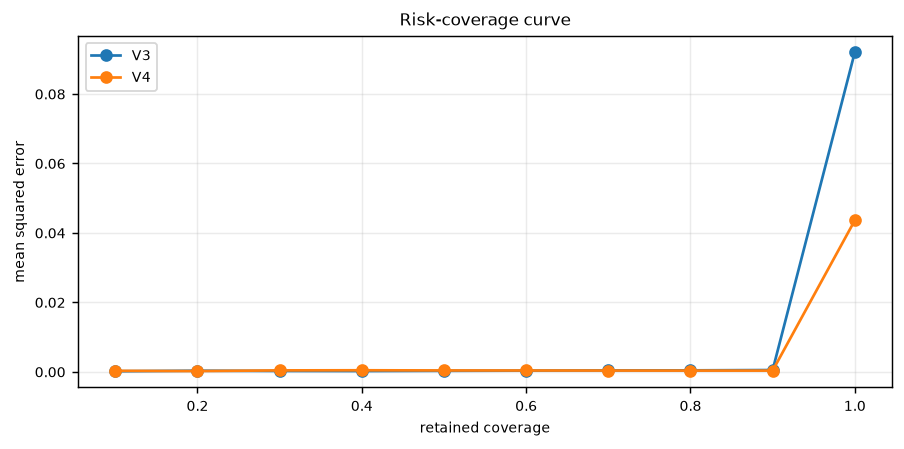
\includegraphics[width=.92\textwidth]{../figures/figure_05_risk_coverage.png}\caption{figure 05 risk coverage}\end{figure}
\begin{figure}[p]\centering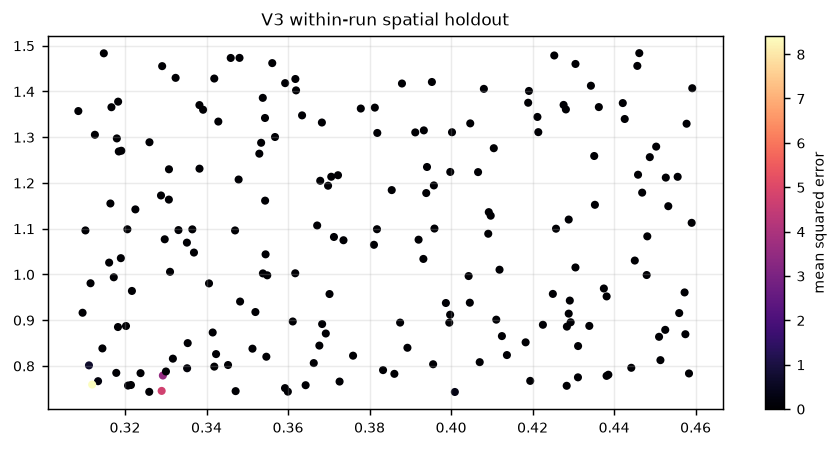
\includegraphics[width=.92\textwidth]{../figures/figure_06_v3_spatial.png}\caption{figure 06 v3 spatial}\end{figure}
\begin{figure}[p]\centering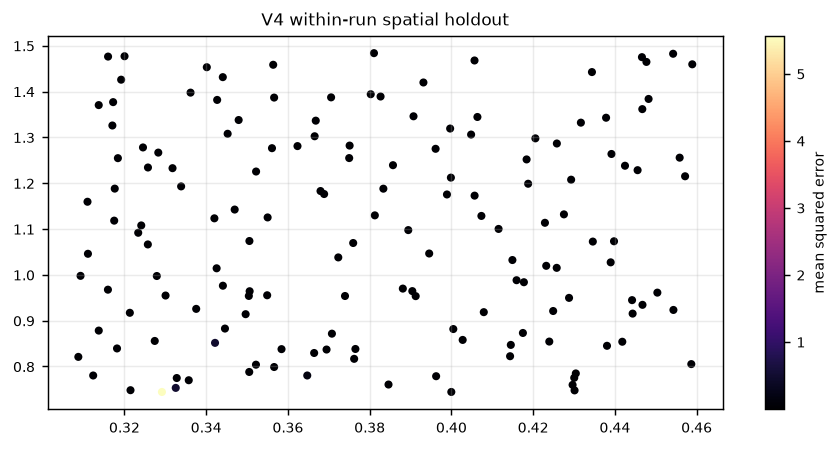
\includegraphics[width=.92\textwidth]{../figures/figure_07_v4_spatial.png}\caption{figure 07 v4 spatial}\end{figure}
\begin{figure}[p]\centering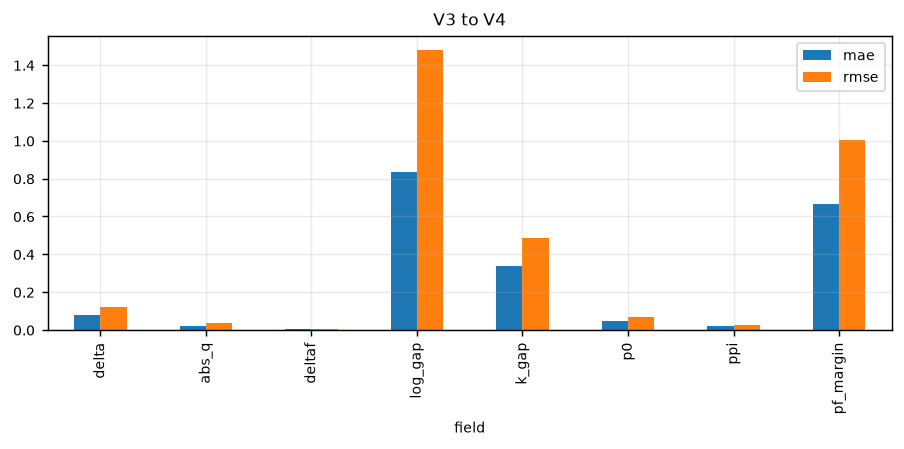
\includegraphics[width=.92\textwidth]{../figures/figure_08_v3_to_v4.png}\caption{figure 08 v3 to v4}\end{figure}
\begin{figure}[p]\centering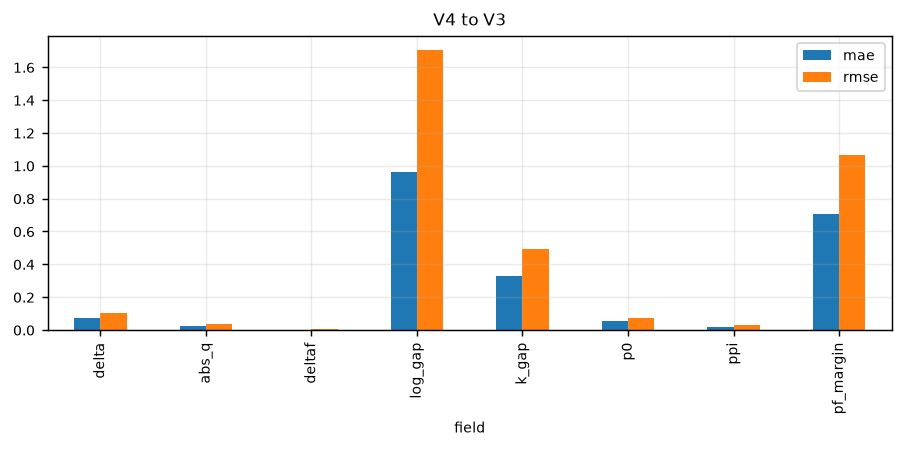
\includegraphics[width=.92\textwidth]{../figures/figure_09_v4_to_v3.png}\caption{figure 09 v4 to v3}\end{figure}
\begin{figure}[p]\centering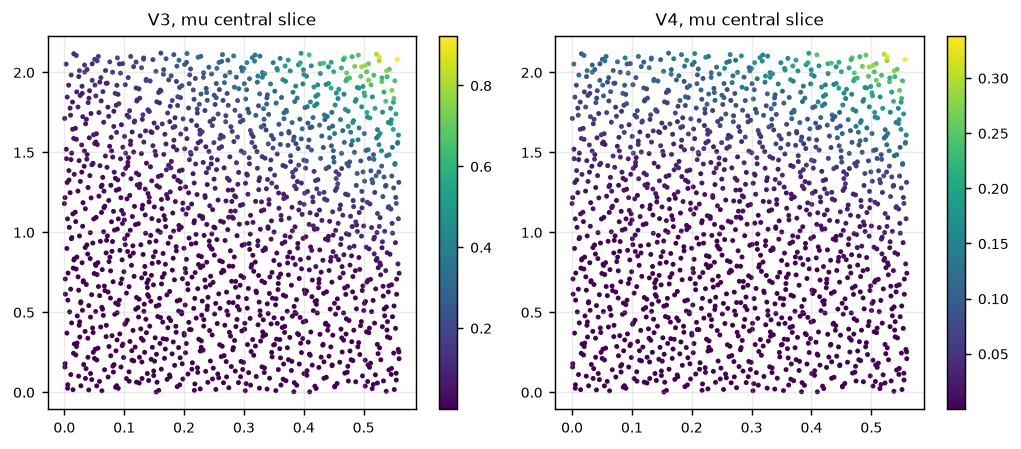
\includegraphics[width=.92\textwidth]{../figures/figure_10_probe_uncertainty.png}\caption{figure 10 probe uncertainty}\end{figure}
\begin{figure}[p]\centering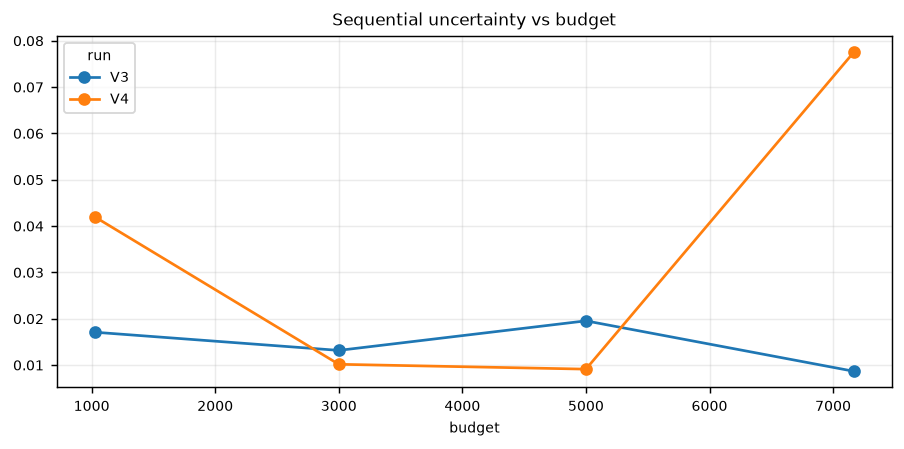
\includegraphics[width=.92\textwidth]{../figures/figure_11_sequential_uncertainty.png}\caption{figure 11 sequential uncertainty}\end{figure}
\begin{figure}[p]\centering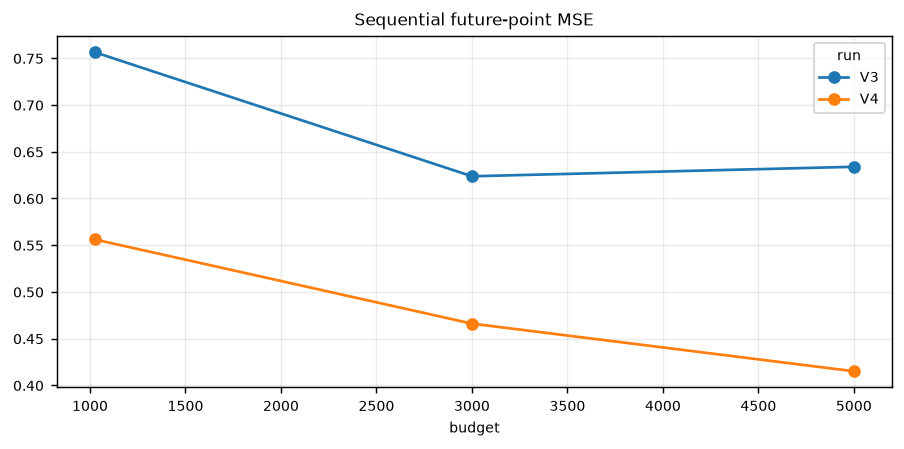
\includegraphics[width=.92\textwidth]{../figures/figure_12_sequential_future_error.png}\caption{figure 12 sequential future error}\end{figure}
\begin{figure}[p]\centering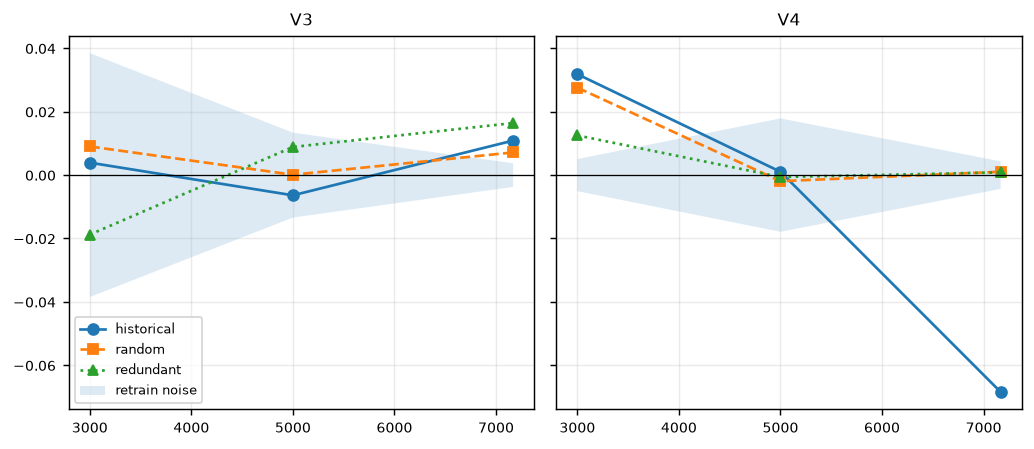
\includegraphics[width=.92\textwidth]{../figures/figure_13_retrospective_information.png}\caption{figure 13 retrospective information}\end{figure}
\begin{figure}[p]\centering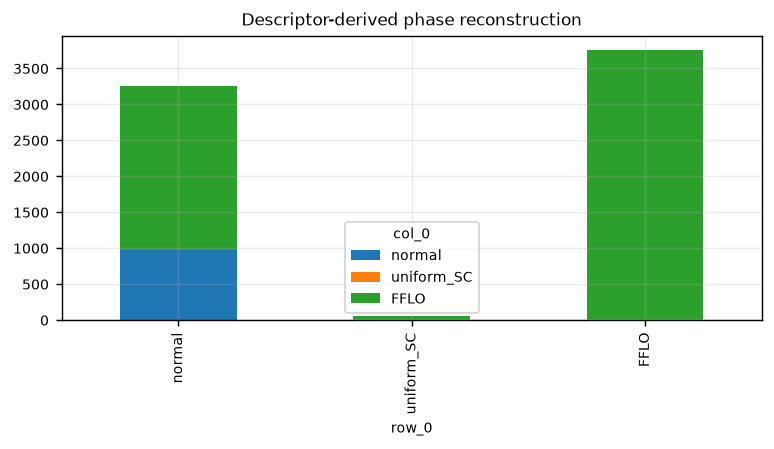
\includegraphics[width=.92\textwidth]{../figures/figure_14_phase_reconstruction.png}\caption{figure 14 phase reconstruction}\end{figure}
\begin{figure}[p]\centering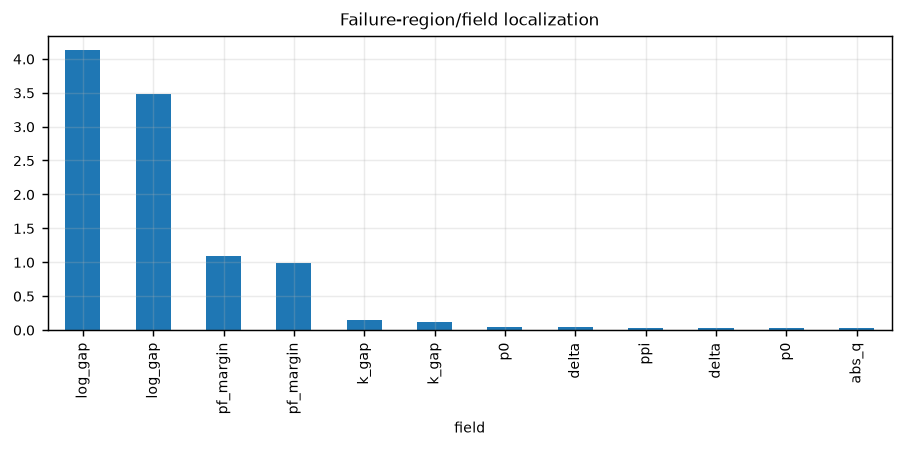
\includegraphics[width=.92\textwidth]{../figures/figure_15_failure_localization.png}\caption{figure 15 failure localization}\end{figure}
\begin{figure}[p]\centering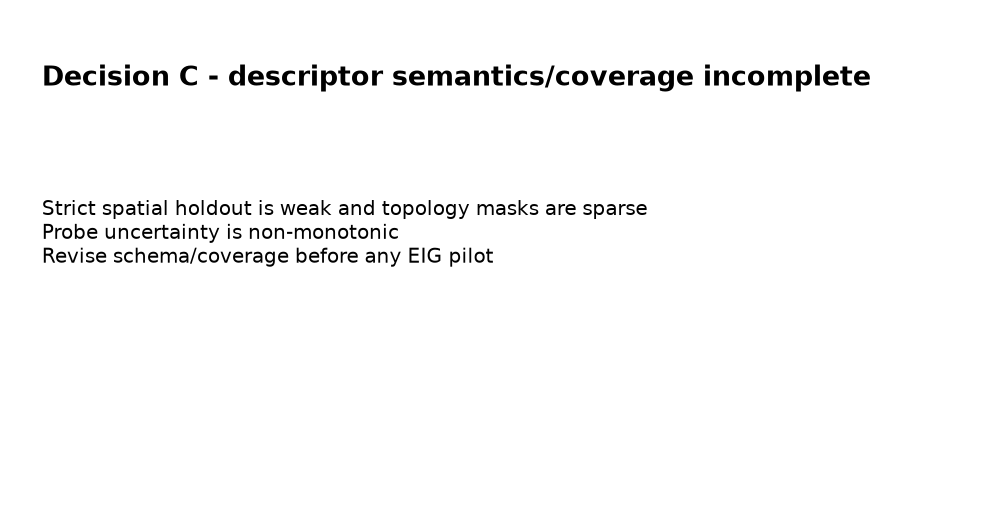
\includegraphics[width=.92\textwidth]{../figures/figure_16_decision_summary.png}\caption{figure 16 decision summary}\end{figure}
\clearpage\section{Production isolation}Only schemas, fixed transforms, architecture, loss source, and tests are allowlisted. Data rows, scalers, checkpoints, weights, optimizer state, latent/cluster state, coordinates, rewards, and replay buffers are denied.\end{document}